% arara: pdflatex: {synctex: yes, action: batchmode, draft: yes, options: "-halt-on-error -file-line-error-style"}
% arara: bibtex
% arara: pdflatex: {synctex: yes, action: batchmode, draft: yes, options: "-halt-on-error -file-line-error-style"}
% arara: pdflatex: {synctex: yes, action: nonstopmode, options: "-halt-on-error -file-line-error-style"}

%% bare_jrnl.tex
%% V1.4a
%% 2014/09/17
%% by Michael Shell
%% see http://www.michaelshell.org/
%% for current contact information.
%%
%% This is a skeleton file demonstrating the use of IEEEtran.cls
%% (requires IEEEtran.cls version 1.8a or later) with an IEEE
%% journal paper.
%%
%% Support sites:
%% http://www.michaelshell.org/tex/ieeetran/
%% http://www.ctan.org/tex-archive/macros/latex/contrib/IEEEtran/
%% and
%% http://www.ieee.org/

%%*************************************************************************
%% Legal Notice:
%% This code is offered as-is without any warranty either expressed or
%% implied; without even the implied warranty of MERCHANTABILITY or
%% FITNESS FOR A PARTICULAR PURPOSE! 
%% User assumes all risk.
%% In no event shall IEEE or any contributor to this code be liable for
%% any damages or losses, including, but not limited to, incidental,
%% consequential, or any other damages, resulting from the use or misuse
%% of any information contained here.
%%
%% All comments are the opinions of their respective authors and are not
%% necessarily endorsed by the IEEE.
%%
%% This work is distributed under the LaTeX Project Public License (LPPL)
%% ( http://www.latex-project.org/ ) version 1.3, and may be freely used,
%% distributed and modified. A copy of the LPPL, version 1.3, is included
%% in the base LaTeX documentation of all distributions of LaTeX released
%% 2003/12/01 or later.
%% Retain all contribution notices and credits.
%% ** Modified files should be clearly indicated as such, including  **
%% ** renaming them and changing author support contact information. **
%%
%% File list of work: IEEEtran.cls, IEEEtran_HOWTO.pdf, bare_adv.tex,
%%                    bare_conf.tex, bare_jrnl.tex, bare_conf_compsoc.tex,
%%                    bare_jrnl_compsoc.tex, bare_jrnl_transmag.tex
%%*************************************************************************


% *** Authors should verify (and, if needed, correct) their LaTeX system  ***
% *** with the testflow diagnostic prior to trusting their LaTeX platform ***
% *** with production work. IEEE's font choices and paper sizes can       ***
% *** trigger bugs that do not appear when using other class files.       ***                          ***
% The testflow support page is at:
% http://www.michaelshell.org/tex/testflow/



\documentclass[journal]{IEEEtran}
%
% If IEEEtran.cls has not been installed into the LaTeX system files,
% manually specify the path to it like:
% \documentclass[journal]{../sty/IEEEtran}





% Some very useful LaTeX packages include:
% (uncomment the ones you want to load)


% *** MISC UTILITY PACKAGES ***
%
%\usepackage{ifpdf}
% Heiko Oberdiek's ifpdf.sty is very useful if you need conditional
% compilation based on whether the output is pdf or dvi.
% usage:
% \ifpdf
%   % pdf code
% \else
%   % dvi code
% \fi
% The latest version of ifpdf.sty can be obtained from:
% http://www.ctan.org/tex-archive/macros/latex/contrib/oberdiek/
% Also, note that IEEEtran.cls V1.7 and later provides a builtin
% \ifCLASSINFOpdf conditional that works the same way.
% When switching from latex to pdflatex and vice-versa, the compiler may
% have to be run twice to clear warning/error messages.






% *** CITATION PACKAGES ***
%
\usepackage{cite}
% cite.sty was written by Donald Arseneau
% V1.6 and later of IEEEtran pre-defines the format of the cite.sty package
% \cite{} output to follow that of IEEE. Loading the cite package will
% result in citation numbers being automatically sorted and properly
% "compressed/ranged". e.g., [1], [9], [2], [7], [5], [6] without using
% cite.sty will become [1], [2], [5]--[7], [9] using cite.sty. cite.sty's
% \cite will automatically add leading space, if needed. Use cite.sty's
% noadjust option (cite.sty V3.8 and later) if you want to turn this off
% such as if a citation ever needs to be enclosed in parenthesis.
% cite.sty is already installed on most LaTeX systems. Be sure and use
% version 5.0 (2009-03-20) and later if using hyperref.sty.
% The latest version can be obtained at:
% http://www.ctan.org/tex-archive/macros/latex/contrib/cite/
% The documentation is contained in the cite.sty file itself.






% *** GRAPHICS RELATED PACKAGES ***
%
\ifCLASSINFOpdf
  \usepackage[pdftex]{graphicx}
  % declare the path(s) where your graphic files are
  % \graphicspath{{../pdf/}{../jpeg/}}
  % and their extensions so you won't have to specify these with
  % every instance of \includegraphics
  % \DeclareGraphicsExtensions{.pdf,.jpeg,.png}
\else
  % or other class option (dvipsone, dvipdf, if not using dvips). graphicx
  % will default to the driver specified in the system graphics.cfg if no
  % driver is specified.
  \usepackage[dvips]{graphicx}
  % declare the path(s) where your graphic files are
  % \graphicspath{{../eps/}}
  % and their extensions so you won't have to specify these with
  % every instance of \includegraphics
  % \DeclareGraphicsExtensions{.eps}
\fi
% graphicx was written by David Carlisle and Sebastian Rahtz. It is
% required if you want graphics, photos, etc. graphicx.sty is already
% installed on most LaTeX systems. The latest version and documentation
% can be obtained at: 
% http://www.ctan.org/tex-archive/macros/latex/required/graphics/
% Another good source of documentation is "Using Imported Graphics in
% LaTeX2e" by Keith Reckdahl which can be found at:
% http://www.ctan.org/tex-archive/info/epslatex/
%
% latex, and pdflatex in dvi mode, support graphics in encapsulated
% postscript (.eps) format. pdflatex in pdf mode supports graphics
% in .pdf, .jpeg, .png and .mps (metapost) formats. Users should ensure
% that all non-photo figures use a vector format (.eps, .pdf, .mps) and
% not a bitmapped formats (.jpeg, .png). IEEE frowns on bitmapped formats
% which can result in "jaggedy"/blurry rendering of lines and letters as
% well as large increases in file sizes.
%
% You can find documentation about the pdfTeX application at:
% http://www.tug.org/applications/pdftex





% *** MATH PACKAGES ***
%
%\usepackage[cmex10]{amsmath}
% A popular package from the American Mathematical Society that provides
% many useful and powerful commands for dealing with mathematics. If using
% it, be sure to load this package with the cmex10 option to ensure that
% only type 1 fonts will utilized at all point sizes. Without this option,
% it is possible that some math symbols, particularly those within
% footnotes, will be rendered in bitmap form which will result in a
% document that can not be IEEE Xplore compliant!
%
% Also, note that the amsmath package sets \interdisplaylinepenalty to 10000
% thus preventing page breaks from occurring within multiline equations. Use:
%\interdisplaylinepenalty=2500
% after loading amsmath to restore such page breaks as IEEEtran.cls normally
% does. amsmath.sty is already installed on most LaTeX systems. The latest
% version and documentation can be obtained at:
% http://www.ctan.org/tex-archive/macros/latex/required/amslatex/math/





% *** SPECIALIZED LIST PACKAGES ***
%
%\usepackage{algorithmic}
% algorithmic.sty was written by Peter Williams and Rogerio Brito.
% This package provides an algorithmic environment fo describing algorithms.
% You can use the algorithmic environment in-text or within a figure
% environment to provide for a floating algorithm. Do NOT use the algorithm
% floating environment provided by algorithm.sty (by the same authors) or
% algorithm2e.sty (by Christophe Fiorio) as IEEE does not use dedicated
% algorithm float types and packages that provide these will not provide
% correct IEEE style captions. The latest version and documentation of
% algorithmic.sty can be obtained at:
% http://www.ctan.org/tex-archive/macros/latex/contrib/algorithms/
% There is also a support site at:
% http://algorithms.berlios.de/index.html
% Also of interest may be the (relatively newer and more customizable)
% algorithmicx.sty package by Szasz Janos:
% http://www.ctan.org/tex-archive/macros/latex/contrib/algorithmicx/




% *** ALIGNMENT PACKAGES ***
%
%\usepackage{array}
% Frank Mittelbach's and David Carlisle's array.sty patches and improves
% the standard LaTeX2e array and tabular environments to provide better
% appearance and additional user controls. As the default LaTeX2e table
% generation code is lacking to the point of almost being broken with
% respect to the quality of the end results, all users are strongly
% advised to use an enhanced (at the very least that provided by array.sty)
% set of table tools. array.sty is already installed on most systems. The
% latest version and documentation can be obtained at:
% http://www.ctan.org/tex-archive/macros/latex/required/tools/


% IEEEtran contains the IEEEeqnarray family of commands that can be used to
% generate multiline equations as well as matrices, tables, etc., of high
% quality.




% *** SUBFIGURE PACKAGES ***
\ifCLASSOPTIONcompsoc
  \usepackage[caption=false,font=normalsize,labelfont=sf,textfont=sf]{subfig}
\else
  \usepackage[caption=false,font=footnotesize]{subfig}
\fi
% subfig.sty, written by Steven Douglas Cochran, is the modern replacement
% for subfigure.sty, the latter of which is no longer maintained and is
% incompatible with some LaTeX packages including fixltx2e. However,
% subfig.sty requires and automatically loads Axel Sommerfeldt's caption.sty
% which will override IEEEtran.cls' handling of captions and this will result
% in non-IEEE style figure/table captions. To prevent this problem, be sure
% and invoke subfig.sty's "caption=false" package option (available since
% subfig.sty version 1.3, 2005/06/28) as this is will preserve IEEEtran.cls
% handling of captions.
% Note that the Computer Society format requires a larger sans serif font
% than the serif footnote size font used in traditional IEEE formatting
% and thus the need to invoke different subfig.sty package options depending
% on whether compsoc mode has been enabled.
%
% The latest version and documentation of subfig.sty can be obtained at:
% http://www.ctan.org/tex-archive/macros/latex/contrib/subfig/




% *** FLOAT PACKAGES ***
%
%\usepackage{fixltx2e}
% fixltx2e, the successor to the earlier fix2col.sty, was written by
% Frank Mittelbach and David Carlisle. This package corrects a few problems
% in the LaTeX2e kernel, the most notable of which is that in current
% LaTeX2e releases, the ordering of single and double column floats is not
% guaranteed to be preserved. Thus, an unpatched LaTeX2e can allow a
% single column figure to be placed prior to an earlier double column
% figure. The latest version and documentation can be found at:
% http://www.ctan.org/tex-archive/macros/latex/base/


%\usepackage{stfloats}
% stfloats.sty was written by Sigitas Tolusis. This package gives LaTeX2e
% the ability to do double column floats at the bottom of the page as well
% as the top. (e.g., "\begin{figure*}[!b]" is not normally possible in
% LaTeX2e). It also provides a command:
%\fnbelowfloat
% to enable the placement of footnotes below bottom floats (the standard
% LaTeX2e kernel puts them above bottom floats). This is an invasive package
% which rewrites many portions of the LaTeX2e float routines. It may not work
% with other packages that modify the LaTeX2e float routines. The latest
% version and documentation can be obtained at:
% http://www.ctan.org/tex-archive/macros/latex/contrib/sttools/
% Do not use the stfloats baselinefloat ability as IEEE does not allow
% \baselineskip to stretch. Authors submitting work to the IEEE should note
% that IEEE rarely uses double column equations and that authors should try
% to avoid such use. Do not be tempted to use the cuted.sty or midfloat.sty
% packages (also by Sigitas Tolusis) as IEEE does not format its papers in
% such ways.
% Do not attempt to use stfloats with fixltx2e as they are incompatible.
% Instead, use Morten Hogholm'a dblfloatfix which combines the features
% of both fixltx2e and stfloats:
%
% \usepackage{dblfloatfix}
% The latest version can be found at:
% http://www.ctan.org/tex-archive/macros/latex/contrib/dblfloatfix/




%\ifCLASSOPTIONcaptionsoff
%  \usepackage[nomarkers]{endfloat}
% \let\MYoriglatexcaption\caption
% \renewcommand{\caption}[2][\relax]{\MYoriglatexcaption[#2]{#2}}
%\fi
% endfloat.sty was written by James Darrell McCauley, Jeff Goldberg and 
% Axel Sommerfeldt. This package may be useful when used in conjunction with 
% IEEEtran.cls'  captionsoff option. Some IEEE journals/societies require that
% submissions have lists of figures/tables at the end of the paper and that
% figures/tables without any captions are placed on a page by themselves at
% the end of the document. If needed, the draftcls IEEEtran class option or
% \CLASSINPUTbaselinestretch interface can be used to increase the line
% spacing as well. Be sure and use the nomarkers option of endfloat to
% prevent endfloat from "marking" where the figures would have been placed
% in the text. The two hack lines of code above are a slight modification of
% that suggested by in the endfloat docs (section 8.4.1) to ensure that
% the full captions always appear in the list of figures/tables - even if
% the user used the short optional argument of \caption[]{}.
% IEEE papers do not typically make use of \caption[]'s optional argument,
% so this should not be an issue. A similar trick can be used to disable
% captions of packages such as subfig.sty that lack options to turn off
% the subcaptions:
% For subfig.sty:
% \let\MYorigsubfloat\subfloat
% \renewcommand{\subfloat}[2][\relax]{\MYorigsubfloat[]{#2}}
% However, the above trick will not work if both optional arguments of
% the \subfloat command are used. Furthermore, there needs to be a
% description of each subfigure *somewhere* and endfloat does not add
% subfigure captions to its list of figures. Thus, the best approach is to
% avoid the use of subfigure captions (many IEEE journals avoid them anyway)
% and instead reference/explain all the subfigures within the main caption.
% The latest version of endfloat.sty and its documentation can obtained at:
% http://www.ctan.org/tex-archive/macros/latex/contrib/endfloat/
%
% The IEEEtran \ifCLASSOPTIONcaptionsoff conditional can also be used
% later in the document, say, to conditionally put the References on a 
% page by themselves.




% *** PDF, URL AND HYPERLINK PACKAGES ***
%
\usepackage{url}
% url.sty was written by Donald Arseneau. It provides better support for
% handling and breaking URLs. url.sty is already installed on most LaTeX
% systems. The latest version and documentation can be obtained at:
% http://www.ctan.org/tex-archive/macros/latex/contrib/url/
% Basically, \url{my_url_here}.




% *** Do not adjust lengths that control margins, column widths, etc. ***
% *** Do not use packages that alter fonts (such as pslatex).         ***
% There should be no need to do such things with IEEEtran.cls V1.6 and later.
% (Unless specifically asked to do so by the journal or conference you plan
% to submit to, of course. )

\usepackage[dutch]{babel}


% *** Do not adjust lengths that control margins, column widths, etc. ***
% *** Do not use packages that alter fonts (such as pslatex).         ***
% There should be no need to do such things with IEEEtran.cls V1.6 and later.
% (Unless specifically asked to do so by the journal or conference you plan
% to submit to, of course. )


\begin{document}
%
% paper title
% Titles are generally capitalized except for words such as a, an, and, as,
% at, but, by, for, in, nor, of, on, or, the, to and up, which are usually
% not capitalized unless they are the first or last word of the title.
% Linebreaks \\ can be used within to get better formatting as desired.
% Do not put math or special symbols in the title.
\title{NanoTorrent: Plaatsbewuste peer-to-peer bestandsdistributie in draadloze sensornetwerken}
%
%
% author names and IEEE memberships
% note positions of commas and nonbreaking spaces ( ~ ) LaTeX will not break
% a structure at a ~ so this keeps an author's name from being broken across
% two lines.
% use \thanks{} to gain access to the first footnote area
% a separate \thanks must be used for each paragraph as LaTeX2e's \thanks
% was not built to handle multiple paragraphs
%
\author{Mattias~Buelens,~\IEEEmembership{KU~Leuven}% <-this % stops a space
\thanks{M. Buelens is een masterstudent aan de KU Leuven, Leuven, Belgi\"e.}}% <-this % stops a space

% note the % following the last \IEEEmembership and also \thanks - 
% these prevent an unwanted space from occurring between the last author name
% and the end of the author line. i.e., if you had this:
% 
% \author{....lastname \thanks{...} \thanks{...} }
%                     ^------------^------------^----Do not want these spaces!
%
% a space would be appended to the last name and could cause every name on that
% line to be shifted left slightly. This is one of those "LaTeX things". For
% instance, "\textbf{A} \textbf{B}" will typeset as "A B" not "AB". To get
% "AB" then you have to do: "\textbf{A}\textbf{B}"
% \thanks is no different in this regard, so shield the last } of each \thanks
% that ends a line with a % and do not let a space in before the next \thanks.
% Spaces after \IEEEmembership other than the last one are OK (and needed) as
% you are supposed to have spaces between the names. For what it is worth,
% this is a minor point as most people would not even notice if the said evil
% space somehow managed to creep in.



% The paper headers
\markboth{augustus~2015}%
{Buelens M.: Plaatsbewuste peer-to-peer bestandsdistributie in draadloze sensornetwerken}
% The only time the second header will appear is for the odd numbered pages
% after the title page when using the twoside option.
% 
% *** Note that you probably will NOT want to include the author's ***
% *** name in the headers of peer review papers.                   ***
% You can use \ifCLASSOPTIONpeerreview for conditional compilation here if
% you desire.




% If you want to put a publisher's ID mark on the page you can do it like
% this:
%\IEEEpubid{0000--0000/00\$00.00~\copyright~2014 IEEE}
% Remember, if you use this you must call \IEEEpubidadjcol in the second
% column for its text to clear the IEEEpubid mark.



% use for special paper notices
%\IEEEspecialpapernotice{(Invited Paper)}


% correct bad hyphenation here
\hyphenation{op-tical net-works semi-conduc-tor}


% make the title area
\maketitle

% As a general rule, do not put math, special symbols or citations
% in the abstract or keywords.
\begin{abstract}

Draadloze sensornetwerken bestaan uit vele kleine computers uitgerust met sensoren en actuatoren die met elkaar kunnen communiceren dankzij hun draadloze antenna. Om deze netwerken operationeel te houden voor lange tijdspannes, moeten ze zich kunnen aanpassen en evolueren ook nadat ze uitgezet zijn in hun omgeving. Dit betekent dat ze grote bestanden zoals nieuwe programma's of configuraties snel en effici\"ent via het netwerk moeten kunnen verkrijgen.

NanoTorrent is een peer-to-peer protocol dat snelle bestandsdistributie toelaat in draadloze sensornetwerken. Het introduceert een hybride mechanisme om peers te vinden, door zowel met een gecentraliseerde tracker te werken en in de lokale omgeving naar buren te zoeken. Dit laat toe om zelfs in zeer heterogene netwerken te opereren, waarbij verschillende knopen verschillende programma's uitvoeren. De peer-to-peer aanpak helpt om de belasting door de bestandsdistributie te verdelen over het netwerk, en maakt gebruik van link-local multicast berichten om delen van het bestand tegelijkertijd naar meerdere buren te distribueren.

De evaluatie van het protocol toont aan dat NanoTorrent een snelle bestandsoverdracht kan realiseren in verschillende netwerkconfiguraties. De hybride aanpak om peers te vinden komt wel met een trade-off waarbij de toegenomen overdrachtssnelheid ook extra transmissies met zich meebrengt. Deze berichten moeten in meerdere hops over het netwerk om afgelegen knopen te bereiken, waardoor de tussenliggende knopen moeten helpen om deze door te sturen. Het protocol kan ook op nog verschillende plaatsen verbeterd worden om minder verkeer over het netwerk te sturen.

\end{abstract}

% Note that keywords are not normally used for peerreview papers.
\begin{IEEEkeywords}
Draadloze sensor netwerken, internet der dingen, peer-to-peer, bestandsdistributie, draadloze netwerken
\end{IEEEkeywords}






% For peer review papers, you can put extra information on the cover
% page as needed:
% \ifCLASSOPTIONpeerreview
% \begin{center} \bfseries EDICS Category: 3-BBND \end{center}
% \fi
%
% For peerreview papers, this IEEEtran command inserts a page break and
% creates the second title. It will be ignored for other modes.
\IEEEpeerreviewmaketitle



\section{Inleiding}
% The very first letter is a 2 line initial drop letter followed
% by the rest of the first word in caps.
% 
% form to use if the first word consists of a single letter:
% \IEEEPARstart{A}{demo} file is ....
% 
% form to use if you need the single drop letter followed by
% normal text (unknown if ever used by IEEE):
% \IEEEPARstart{A}{}demo file is ....
% 
% Some journals put the first two words in caps:
% \IEEEPARstart{T}{his demo} file is ....
% 
% Here we have the typical use of a "T" for an initial drop letter
% and "HIS" in caps to complete the first word.
\IEEEPARstart{D}{raadloze} sensornetwerken zijn een opkomende vorm van computernetwerken bestaande uit vele kleine computers met beperkte mogelijkheden en capaciteiten die uitgerust zijn met allerlei sensoren en actuatoren en met elkaar draadloos kunnen communiceren. Deze computers of `knopen' werken samen om metingen te verrichten, gegevens te verzamelen en te verwerken en acties te plannen en uit te voeren. Draadloze sensornetwerken kunnen uitgezet worden in voor mensen moeilijk bereikbare of gevaarlijke omgevingen, zoals in metrotunnels of op vulkanen \cite{reventador}. Hier kunnen ze wetenschappelijke metingen doen, gevaren in de omgeving detecteren of zelf beslissen om actie te ondernemen.

Omdat deze netwerken voor lange tijd moeten meegaan en mogelijk niet meer fysiek toegankelijk zijn nadat ze zijn ge\"installeerd, moeten ze kunnen aangepast worden op afstand. Nieuwe toepassingen of nieuwe taakconfiguraties moeten kunnen verspreid worden naar alle knopen in het netwerk, en deze moeten zich zelfstandig kunnen herconfigureren met de nieuwe data. Deze herprogrammering of herconfiguratie van het netwerk moet liefst zo snel mogelijk gebeuren, zodat de knopen kunnen verder gaan met hun eigenlijke taak. Omdat de kleine computers vaak op batterijen werken, moet dit ook energie-effici\"ent gebeuren met zo weinig mogelijk uitgewisselde berichten tussen knopen.

NanoTorrent is een peer-to-peer protocol dat zulke grote bestanden kan verspreiden over een draadloos sensor netwerk. Hiervoor gebruikt het een hybride mechanisme om peers te vinden, door zowel met een gecentraliseerde tracker te werken en in de lokale omgeving naar buren te zoeken. De peer-to-peer bestandsoverdracht helpt om de belasting van de gecommuniceerde berichten te verdelen over het hele netwerk.

Het vervolg van dit artikel is als volgt gestructureerd. Sectie \ref{sec:context} geeft een overzicht van de probleemcontext van internet der dingen en draadloze sensornetwerken. Sectie \ref{sec:ontwerp} bespreekt het ontwerp van het NanoTorrent protocol. Sectie \ref{sec:implementatie} beschouwt de implementatie van het gemaakte prototype. Sectie \ref{sec:evaluatie} evalueert het ontwerp en het prototype. Sectie \ref{sec:gerelateerd} bespreekt het onderzochte gerelateerde werk. Sectie \ref{sec:conclusies} eindigt het artikel met de conclusies.

\section{Context}
\label{sec:context}

\subsection{Internet der dingen}
In de visie van het `internet der dingen' worden fysieke objecten uitgerust met kleine ingebouwde computers die het mogelijk maken om deze dingen te monitoren en te besturen op elk moment van eender waar ter wereld. Dankzij IPv6 kan ieder object een uniek adres toegewezen worden dat via het internet bereikbaar is \cite{iotcluster15}.

De mogelijke toepassingen van het internet der dingen beslaan bijna alle domeinen, gaande van het verbeteren van het comfort thuis tot het controleren van grote essenti\"ele infrastructuren:

\emph{Slimme huizen.} Door huishoudtoestellen, temperatuursensoren en beveiligingscamera's te verbinden met het internet, kan een huiseigenaar op ieder moment zijn leefcomfort controleren met elk toestel \cite{chan-smart-home-review}. Met een enkel dashboard krijgt hij een overzicht van alle toestellen thuis, en kan hij bijvoorbeeld zowel de airconditioning als de rolluiken aansturen.

\emph{Slimme elektriciteitsnetten.} Met de verschuiving van fossiele brandstoffen naar hernieuwbare energiebronnen wordt energieproductie steeds minder voorspelbaar. Terwijl kool- en kerncentrales elektriciteit kunnen produceren op ieder moment, hangt de productie van zonnepanelen en windmolenparken af van de tijd en de weercondities. Dit kan leiden tot tekorten of blackouts, of overproductie. Om te kunnen omgaan met deze fluctuaties, moeten slimme elektriciteitsnetten de mogelijkheid hebben om het energieverbruik nauwkeuriger te voorspellen op korte termijn, en om verbruikspieken te verschuiven naar momenten waarop er meer productiecapaciteit is \cite{gungor-smart-grid-survey}. Huizen kunnen uitgerust worden met slimme elektriciteitsmeters die continue het verbruik meten en doorsturen naar de producenten, en wasmachines kunnen geprogrammeerd worden om te werken wanneer er weinig verbruik op het net is. Dit biedt veel uitdagingen om een gesofisticeerde IT infrastructuur te ontwikkelen die deze slimme apparaten kan ondersteunen \cite{gungor-smart-grid-technologies}, zoals getoond in figuur \ref{fig:context:smart-grid}.

\begin{figure}
    \centering
    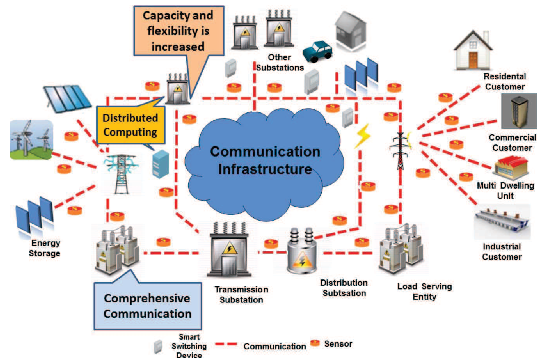
\includegraphics[width=\linewidth]{images/smart-grid-architecture.pdf}
    \caption{Voorbeeld van een architectuur voor een slim elektriciteitsnet. \cite{gungor-smart-grid-technologies}}
    \label{fig:context:smart-grid}
\end{figure}

\subsection{Draadloze sensornetwerken}
Vele toepassingen in het internet der dingen worden ge\"implementeerd met een draadloos sensornetwerk. Deze bestaan uit een aantal kleine computers (ook wel `knopen' of `motes' genoemd) met sensoren, actuatoren en een draadloze antenne. De knopen meten veranderingen in hun omgeving, communiceren met elkaar en de buitenwereld en werken in op hun omgeving.

Knopen in een draadloos sensornetwerken verschillen sterk van gewone computers, en hebben verschillende ontwerpvereisten voor hun programma's:
\begin{itemize}
\item Door hun kleine grootte zijn ze beperkt in hun mogelijkheden. Terwijl gewone computers multi-core gigahertz processors hebben met RAM geheugen in de orde van GB, hebben knopen slechts megahertz microprocessoren en een paar KB aan RAM. De TMote Sky heeft bijvoorbeeld een kloksnelheid van 8 MHz en 48 KB aan geheugen \cite{tmote-sky-manual}, terwijl de AVR Zigduino r2 (figuur \ref{fig:context:zigduino}) aan 16 MHz draait met 128 KB aan flash RAM \cite{zigduino-manual}.
\item De levensduur van een knoop is beperkt door zijn batterij. Dit maakt energieverbruik een belangrijke ontwerpvereiste voor programmeurs.
\item Draadloze sensor netwerken zijn onbetrouwbaar. Knopen kunnen falen doordat hun batterij opgebruikt zijn of doordat de omgeving hen fysiek vernielt (overstromingen, branden, aardbevingen,...) Programmeurs moeten rekening houden met falende knopen.
\item Draadloze netwerken zijn erg gedistribueerd. Een netwerk kan bestaan uit honderden knopen, met mobiele knopen die binnen en buiten het bereik van de antenne vallen. Gedistribueerde programma's moeten kunnen schalen naar zulke grote aantallen van knopen.
\end{itemize}

\begin{figure}
	\centering
	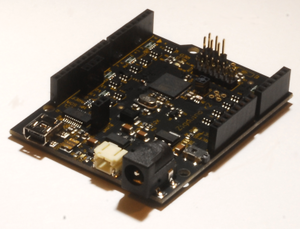
\includegraphics[width=\linewidth]{images/zigduino-r2.png}
	\caption{Het AVR Zigduino r2 platform. \cite{zigduino-manual}}
	\label{fig:context:zigduino}
\end{figure}

\subsection{BitTorrent}
Het voorgestelde protocol haalt veel inspirate van het BitTorrent protocol \cite{bep3}. Dit is een peer-to-peer bestandsdistributieprotocol voor het internet, dat het bestand opsplitst in gelijke delen (`pieces') die afzonderlijk verspreid kunnen worden tussen peers. Gebruikers moeten eerst een \texttt{.torrent} bestand downloaden om de eigenlijke distributie van de `torrent' te starten in hun BitTorrent client.

Peers melden zich aan bij een centrale tracker, die hun deelname registreert in de `swarm' en een lijst van andere peers terug geeft. Peers kunnen vervolgens verbinding maken met de ontdekte peers, en ontdekken welke pieces de andere peers al hebben gedownload. Een peer kan dan een piece dat hij ontbreekt aanvragen bij een andere peer, het piece ontvangen en vervolgens zelf verspreiden naar andere peers.

BitTorrent zorgt ervoor dat peers ook moeten helpen met pieces te uploaden, en niet enkel mogen downloaden. Hiervoor gebruikt het een tit-for-tat strategie, waarbij peers die weigeren om pieces aan te bieden gestrafd worden doordat andere peers ook zullen weigeren om pieces aan te bieden aan deze slechte peer. Dit maakt dat alle peers verplicht worden te helpen bij de distributie, en zo de belasting over de verschillende peers eerlijker verdeeld wordt.

NanoTorrent neemt de concepten van torrents, trackers, swarms en pieces over in het ontwerp. Peers worden op een gelijkaardige manier gevonden via een tracker, en bestanden worden als pieces verspreid over het peer-to-peer netwerk.

\section{Ontwerp}
\label{sec:ontwerp}
Het ontwerp van het NanoTorrent protocol bestaat uit twee grote delen: het vinden van peers om mee te verbinden, en het uitwisselen van het bestand met deze gevonden peers.

\subsection{Vinden van peers}
NanoTorrent gebruikt twee parallele mechanismen om peers te vinden.

\emph{Peers vinden met tracker.} Een eerste manier bestaat erin om peers te laten communiceren met een centrale `tracker', die bijhoudt welke peers er momenteel deelnemen aan de distributie van de torrent. Wanneer de tracker een aanvraag ontvangt van een peer, voegt hij deze peer toe aan de swarm en geeft als antwoord een aantal andere peers uit dezelfde swarm terug. De peer kan dan verbindingen beginnen maken met peers uit de ontvangen lijst. Opdat de tracker geen peers teruggeeft die al lang niet meer reageren en dus geen verbindingen zullen accepteren van peers, moeten peers periodiek hun deelname bij de tracker vernieuwen. De tracker kan dan oude peers na een tijd verwijderen, zodat deze niet meer voorkomen in de antwoorden.

\emph{Lokale peers.} Een tweede manier gebruikt de nabijheid van andere peers om deze te vinden. Peers sturen periodiek een bericht naar alle buren in hun omgeving met informatie over de torrent die zij momenteel aan het downloaden zijn. Hiervoor maken zij gebruik van IPv6 link-local multicast berichten. Wanneer een peer zo'n multicast bericht ontvangt, kan hij zien van welke buur dit bericht kwam en zelf een verbinding beginnen met deze buur. Doordat berichten over een draadloos medium hoe dan ook hoorbaar moeten zijn voor alle omringende buren, kost het verzenden van zo'n multicast bericht even veel als een gewoon unicast bericht gericht naar slechts \'e\'en ontvanger.

Door deze twee mechanismen samen te gebruiken, kan het protocol meer heterogene draadloze netwerken ondersteunen bestaande uit een aantal clusters van knopen. Binnen een cluster kunnen knopen elkaar vinden met lokale berichten, terwijl ze knopen uit andere clusters kunnen vinden via het antwoord van de tracker.

\subsection{Bestandsdistributie}
De peer-to-peer bestandsdistributie is erg gelijkaardig aan dat van BitTorrent. Het heeft wel enkele belangrijke aanpassingen met het oog op de beperkte capaciteiten van knopen in een draadloos sensornetwerk.

Peers proberen verbindingen op te zetten met alle peers die ze weten te vinden. Voor elke verbinding moeten ze een beetje geheugen reserveren om de toestand bij te houden. Deze toestand bestaat uit: het IPv6 adres van de andere peer, de set van pieces die beschikbaar zijn bij de andere peer, het tijdstip van het laatste bericht ontvangen van deze peer, en informatie over de huidige aanvraag voor een piece die onlangs verstuurd is naar de peer. Peers onderhouden hun verbindingen door periodiek \texttt{have} berichten te versturen, waarin ze hun huidige set van beschikbare pieces meedelen aan verbonden peers. De ontvangende peers werken dan hun beeld op de toestand van die peer bij.

Wanneer een peer merkt dat een ontbrekende piece beschikbaar is geworden bij een van zijn verbonden peers, kan deze een aanvraag versturen voor die piece. De peer verstuurt als antwoord de inhoud van die piece, zodat de ontvanger deze data kan wegschrijven en zelf de piece kan aanbieden aan zijn eigen connecties.

Als optimalizatie kunnen peers die een aanvraag voor een piece ontvangen van een lokale peer, hun antwoord met de data versturen naar \emph{alle} buren als een multicast bericht. Dit laat lokale peers toe om data te ontvangen voor pieces die zij nog niet expliciet hadden aangevraagd, maar wel in ge\"intereseerd zijn. Zo kan een lokale piece uitwisseling meerdere lokale peers tegelijk bedienen.

\section{Implementatie}
\label{sec:implementatie}
De systeemarchitectuur van de implementatie van het prototype is weergegeven in figuur \ref{fig:impl:architecture}. Hierin is de tracker verantwoordelijk voor het beheer van de swarm, de peer verantwoordelijk voor het vinden van andere peers en het uitwisselen van pieces, en de border router verantwoordelijk voor de verbinding tussen het draadloze sensornetwerk en het externe netwerk waar de tracker zich bevindt.

\subsection{Tracker}
De tracker is ge\"implementeerd als een stand-alone Java applicatie. Peers communiceren met de tracker over het NanoTracker UDP protocol om deel te nemen aan een swarm en peers te vinden in de swarm. De tracker onderhoudt de toestand van alle swarms en alle peers die hij opvolgt, en gebruikt deze informatie om een lijst van andere peers in de swarm aan te bieden aan nieuwe peers. In de huidige versie van het prototype kiest de tracker gewoon een aantal peers uit de swarm willekeurig, zonder een intelligent selectie algoritme. Dit kan indien nodig aangepast worden om meer informatie in rekening te houden bij deze keuze, zodat peers betere verbindingen kunnen opzetten.

\subsection{Peer}
De peer is ge\"implementeerd in C als een Contiki \cite{contiki} applicatie. Deze moet o.a. de verbinding met de tracker onderhouden, verbindingen met peers maken en accepteren, pieces kiezen om aan te vragen bij andere peers en op zijn beurt pieces aanbieden aan andere peers.

Om te vermijden dat peers te veel connecties tegelijkertijd zouden openen, zijn het aantal tegelijk geopende connecties beperkt. Wanneer een peer een nieuwe connectie probeert te openen, kan het dus zijn dat dit mislukt. De peer stuurt een \texttt{close} message sturen naar de andere peer om te laten weten dat hij de connectie niet kon openen, zodat deze aan zijn kant de eigen toestand ook kan opkuisen.

Peers gebruiken net zoals BitTorrent een \emph{zeldzaamste eerst} policy om pieces te selecteren voor aanvragen. Hierbij verkiest de peer om eerst de piece aan te vragen die het minst voorkomen bij zijn verbonden peers. Dit helpt om deze zeldzame pieces sneller te verspreiden over de rest van het netwerk, zodat ze sneller minder zeldzaam worden en de belasting op het netwerk weer beter verdeeld kan worden.

Peers zorgen er ook voor dat ze eenzelfde piece niet bij meerdere peers tegelijk aanvragen. Dit is ineffici\"ent, omdat de peer beter verschillende pieces in parallel kan aanvragen. Een uitzondering op deze regel is wanneer de peer bijna alle pieces heeft gedownload. In deze \emph{end-game modus} tracht de peer zo snel mogelijk de paar ontbrekende pieces te downloaden met meerdere aanvragen bij verschillende peers, zodat de peer sneller het volledige bestand heeft en andere peers optimaal kan helpen met hun distributie.

Pieces worden opgeslagen in het Contiki File System (CFS). Afhankelijk van het platform waarvoor de Contiki applicatie wordt gecompileerd, kan dit belanden op een harde schijf, een EEPROM geheugen of in RAM geheugen. Op het AVR Zigduino platform kan CFS naar 4 KB aan EEPROM geheugen schrijven \cite{zigduino-manual}. CFS maakt abstractie van deze verschillende opslagmedia, en biedt een uniforme interface om bestanden te lezen en te schrijven.

\begin{figure}
    \centering
    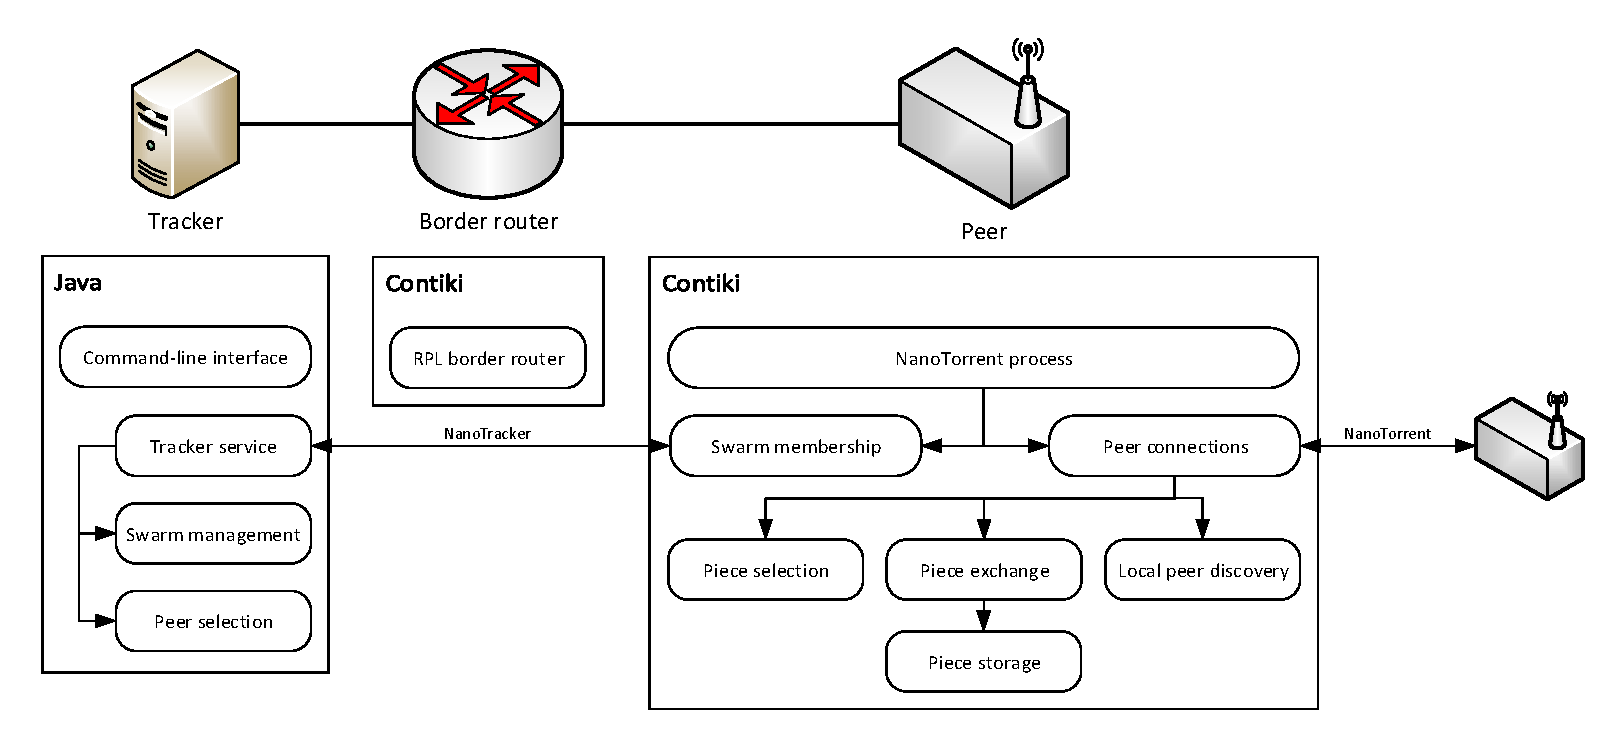
\includegraphics[width=\linewidth]{diagrams/protocol-architecture.pdf}
    \caption{NanoTorrent systeemarchitectuur}
    \label{fig:impl:architecture}
\end{figure}

\section{Evaluatie}
\label{sec:evaluatie}
Het prototype werd ge\"evalueerd op zijn schaalbaarheid en op zijn bruikbaarheid in een heterogene netwerkconfiguratie door middel van de COOJA simulator.

Het doel van NanoTorrent is om bestanden te distribueren naar vele knopen in een draadloos netwerk, in een aanvaardbare tijd en met zo weinig mogelijk berichten om energie-effici\"ent te zijn op fysieke knopen. Het moet bruikbaar zijn in verschillende netwerkconfiguraties bestaande uit verschillende soorten knopen met verschillende programma's, die mogelijk niet allemaal deelnemen aan de NanoTorrent distributie.

COOJA \cite{cooja} maakt het mogelijk om een volledig Contiki platform te simuleren zonder wijzigingen aan de code van de geteste applicatie. In de simulator kan eender welke configuratie van knopen getest worden, met verschillende parameters voor het communicatiemedium. Tijdens de simulatie kan alle uitvoer en verzonden pakketten weergegeven en opgeslagen worden, wat zeer nuttig is om later analyses te maken.

\subsection{Schaalbaarheid}
De schaalbaarheid van het protocol werd getest door een bestand te distribueren in een netwerk met $N^2$ knopen in een $N \times N$ rasterconfiguratie, zoals in figuur \ref{fig:eval:scale:setup}. De resultaten zijn getoond in figuur \ref{fig:eval:scale:deploy-time} en \ref{fig:eval:scale:total-transmissions}.

Het gebruik van een tracker zorgt duidelijk voor een snellere distributie, doordat peers meer verbindingen kunnen maken en zo sneller pieces kunnen aanvragen. Zonder een tracker moeten peers wachten totdat hun onmiddellijke buren pieces beginnen te ontvangen.

Echter, de toegenomen distributiesnelheid zorgt voor een drastische toename in het aantal verzonden berichten. Omdat peers communiceren met ver afgelegen peers ontdekte via de tracker, moeten hun berichten langs meerdere tussenliggende knopen passeren vooraleer ze hun bestemming bereiken. Deze tussenliggende knopen moeten hun eigen energie gebruiken om deze extra berichten door te sturen naar de juiste bestemming, wat zorgt voor meer verkeer op het netwerk. Wanneer de tracker niet gebruikt wordt, blijft het aantal verzonden berichten veel meer beperkt en schaalt het beter naarmate het netwerk groter wordt.

\begin{figure}
    \centering
    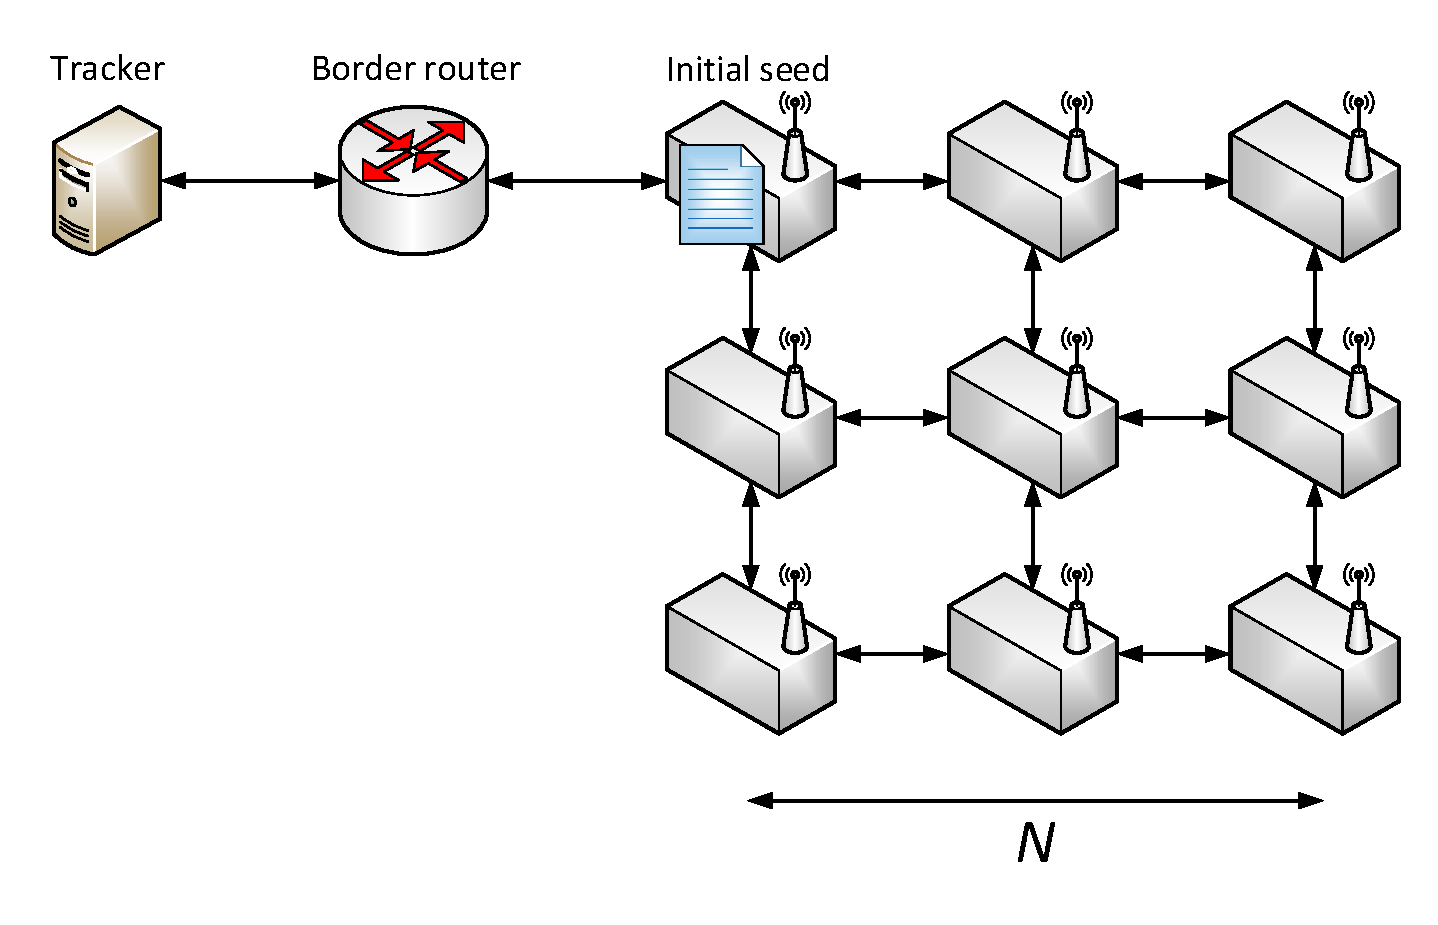
\includegraphics[width=\linewidth]{diagrams/experiment-scale.pdf}
    \caption{Netwerkconfiguratie voor schaalbaarheidsexperiment. Het netwerk bestaat uit $N \times N$ knopen uitgelijnd in een raster, met \'e\'en initi\"ele seed.}
    \label{fig:eval:scale:setup}
\end{figure}

\begin{figure}
    \centering
    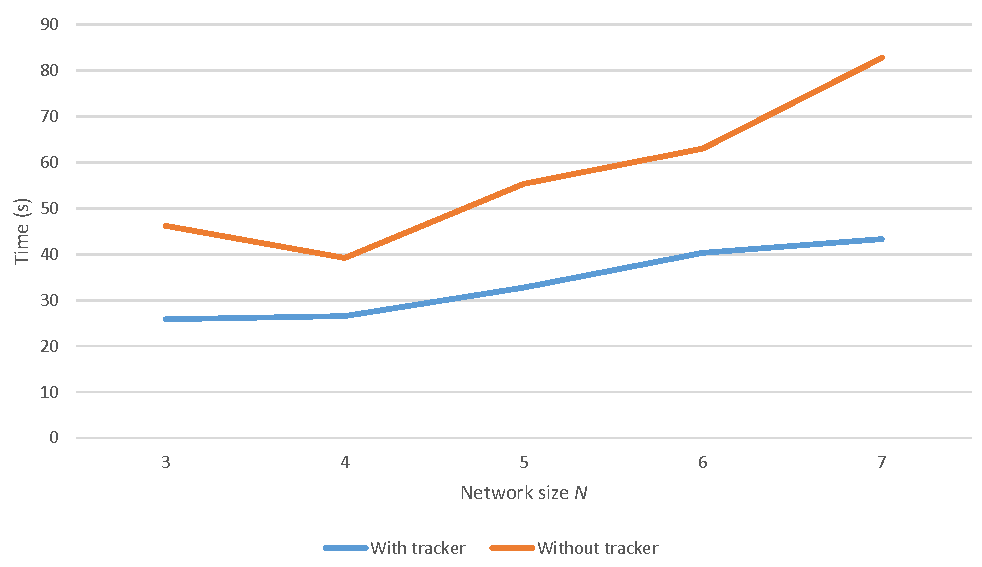
\includegraphics[width=\linewidth]{graphs/scale/deploy-time.pdf}
    \caption{Tijd nodig om het volledige bestand te distribueren naar alle knopen voor een netwerkdiameter $N$.}
    \label{fig:eval:scale:deploy-time}
\end{figure}

\begin{figure}
    \centering
    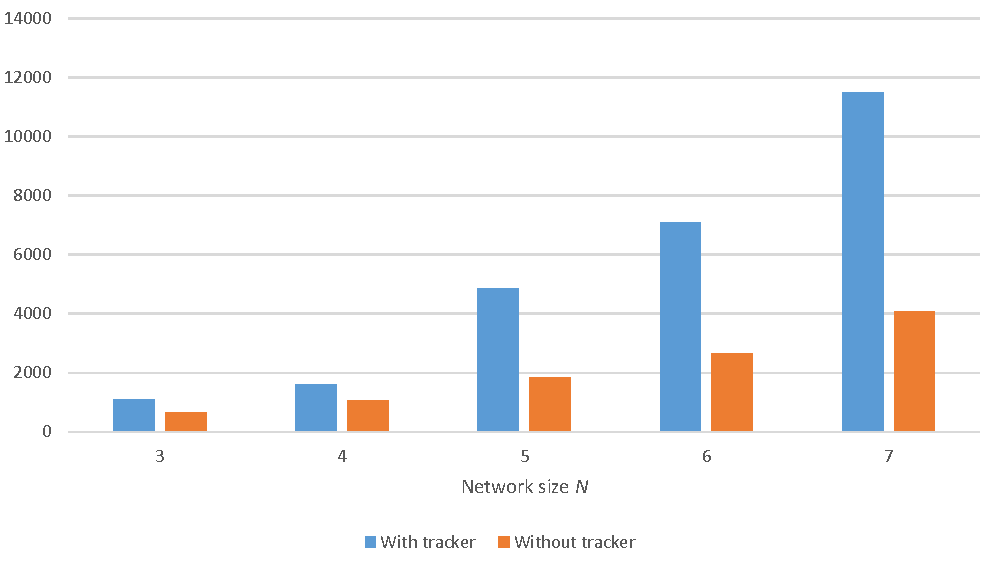
\includegraphics[width=\linewidth]{graphs/scale/total-transmissions.pdf}
    \caption{Total aantal transmissies verzonden tijdens de distributie voor een toenemende netwerkdiameter $N$.}
    \label{fig:eval:scale:total-transmissions}
\end{figure}

\subsection{Heterogeniteit}
Terwijl andere protocols zoals Deluge \cite{deluge} vereisen dat alle knopen in het netwerk hetzelfde protocol draaien, kan NanoTorrent opereren in heterogene netwerken waarbij sommige knopen geen NanoTorrent implementatie uitvoeren.

Om deze toepassing te valideren, werd een experiment uitgevoerd met twee clusters van $5 \times 5$ knopen die enkel verbonden worden door een border router. De initi\"ele seed werd geplaatst in \'e\'en van de twee clusters, zodat peers in de andere cluster moeten verbindingen maken met deze cluster om het bestand te kunnen verkrijgen.

De verdeling van de voltooiingstijden van de verschillende peers is getoond in figuur \ref{fig:eval:hetero:completion}. Hieruit blijkt dat het tot een minuut duurt vooraleer de eerste knoop in de andere cluster het volledige bestand heeft ontvangen. Zodra de eerste knoop in deze cluster de download heeft voltooid, kan het bestand wel sneller verspreiden doorheen de cluster, zodat alle knopen na in totaal anderhalve minuut het volledige bestand hebben.

\begin{figure}
	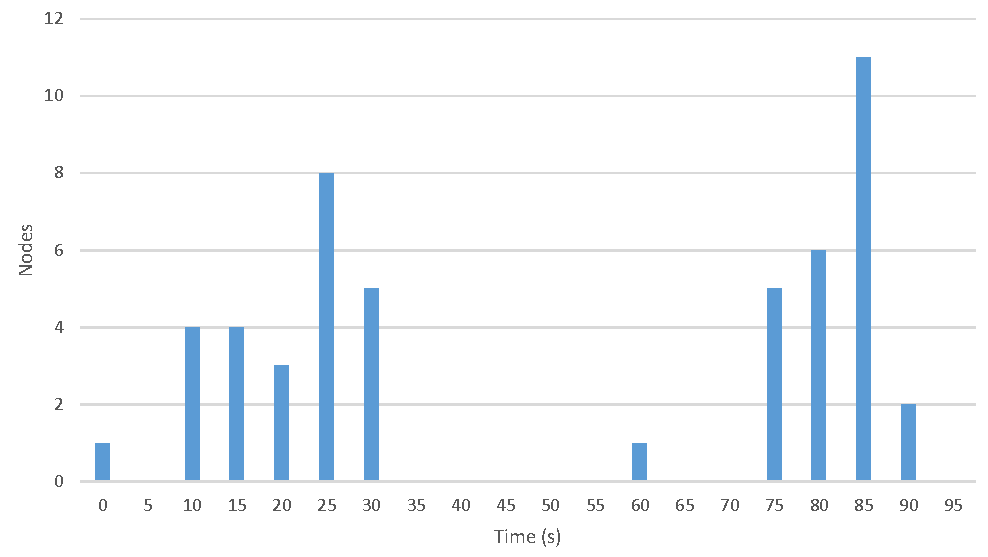
\includegraphics[width=\linewidth]{graphs/cluster/two-cluster-seed-12-completion.pdf}
	\caption{Voltooiingstijden in netwerk met twee $5 \times 5$ clusters.}
	\label{fig:eval:hetero:completion}
\end{figure}

\subsection{Mogelijke verbeteringen}
Er is duidelijk nog ruimte voor verbetering aan het protocol. Zeker het aantal verzonden berichten bij het gebruik van een tracker moet nog effici\"enter gemaakt worden om bruikbaar te zijn in echte draadloze netwerken.

De configuratieparameters van het protocol moeten nog beter fijngesteld worden. Deze bepalen o.a. de waarden van de timers en het aantal tegelijk geopende connecties, die een grote impact kunnen hebben op de performantie. Periodieke \texttt{have} berichten kunnen initieel sneller verstuurd worden om sneller te kunnen beginnen met pieces te verspreiden. Momenteel is er ook nog weinig co\"ordinate tussen knopen bij het versturen van aanvragen voor pieces, in vergelijking met Deluge \cite{deluge} dat redundante aanvragen zoveel mogelijk tracht te vermijden.

Het is ook nog mogelijk dat peers twee verbindingen maken met dezelfde peer. Peers kunnen niet achterhalen of een peer gevonden via een tracker en via lokale multicast aankondigingen dezelfde fysieke node draaien.

\subsection{Discussie}
Uit de resultaten van het schaalbaarheidsexperiment volgt dat het gebruik van een tracker een trade-off met zich meebrengt. De distributiesnelheid kan verhoogd worden, ten koste van meer berichten over het netwerk.

NanoTorrent laat echter wel toe om in meer netwerkconfiguraties bestanden te distribueren doordat het IPv6 gebruikt als onderliggend netwerkprotocol. Het heterogeniteitsexperiment toont aan dat NanoTorrent een bestand kan distribueren tussen twee clusters gescheiden door een IPv6 border router, iets waar andere protocollen niet in slagen.

\section{Gerelateerd werk}
\label{sec:gerelateerd}

\subsection{Local Peer Discovery for BitTorrent}
Local Peer Discovery \cite{bt-ldp} is een uitbreiding voor BitTorrent die peers toelaat om andere peers te vinden op het lokale netwerk (LAN). Hiervoor gebruikt het speciale multicast aankondigingen die niet buiten het lokale netwerk gerouteerd worden. Een peer kondigt aan welke torrent hij aan het downloaden is, zodat andere luisterende peers een verbinding kunnen openen met deze peer.

In de praktijk wordt deze uitbreiding weinig gebruikt in BitTorrent. Het is weinig waarschijnlijk dat twee gebruikers op een thuisnetwerk tegelijk dezelfde torrent zullen downloaden, en op een bedrijfsnetwerk wordt BitTorrent vaak niet toegelaten. In de context van draadloze sensornetwerken is het wel zeer relevant, en daarom is het opgenomen in aangepaste vorm in het NanoTorrent protocol.

\subsection{Deluge}
Deluge \cite{deluge} is een protocol om bestanden te distribueren in een draadloos sensornetwerk.

Knopen kondigen periodiek aan welke versie van het bestand ze hebben, en luisteren naar meldingen van hun buren. Wanneer ze ontdekken dat een buur een nieuwe versie heeft, sturen ze een aanvraag voor de delen van dit bestand. Buren met delen van dit bestand kunnen dan hun data verspreiden naar ge\"interesseerde buren.

Het gebruikt Trickle timers \cite{trickle} om effici\"ent lokale broadcasts te versturen naar buren. Iedere knoop luistert eerst een tijdje naar wat andere buren versturen alvorens zelf een bericht te sturen. Als ze merken dat verschillende buren reeds een identiek bericht hebben verstuurd, is het niet nodig dat de knoop dat bericht nog eens herhaald. De knoop kan zo besparen op zijn transmissie.

Deluge neemt dus gretig gebruik van de effici\"entie van lokale broadcasts in draadloze sensornetwerken. De idee\"en kunnen ook gebruikt worden voor piece uitwisseling met lokale peers in NanoTorrent, maar vertalen moeilijk naar ver afgelegen peers gevonden via de tracker. Om het ontwerp van het prototype eenvoudig te houden, zijn de optimalisaties van Deluge  voorlopig niet ge\"implementeerd in NanoTorrent.

\subsection{TinyTorrents}
TinyTorrents \cite{tinytorrents} is een peer-to-peer protocol om torrents te verspreiden in een draadloos sensornetwerk. Het is sterk ge\"inspireerd door BitTorrent, en gebruikt ook torrent files, trackers en pieces.

De auteurs van TinyTorrents herkennen vele van de uitdagingen van draadloze sensornetwerken in de problemen die BitTorrent oplost. BitTorrent tracht de belasting op het netwerk evenwichtig te houden, verifieert de integriteit van pieces met checksums en maakt distributie snel en effici\"ent met de zeldzaamste-eerste policy voor pieces. Mede daarom komen deze concepten ook terug in het ontwerp van NanoTorrent.

TinyTorrents biedt ook compatibiliteit met gewone BitTorrent door middle van een gateway die de brug spant tussen beide protocollen. Hoewel dit interessant is om sensormetingen beschikbaar te maken aan BitTorrent clients op het internet, is het niet echt nuttig om bestanden te sturen naar een draadloos sensornetwerk.

\subsection{Uitdagingen en aanpakken voor het herprogrammeren van draadloze sensornetwerken}
Wang et al. \cite{wang-reprogramming} schetsen een raamwerk om de verschillende functies nodig in een oplossing voor het herprogrammeren van sensornetwerken te onderzoeken. Hun framework omvat functies zoals versiebeheer, selectie van scopes, en aanvragen van code. Een protocol voor bestandsdistributie zoals NanoTorrent kan hierin de functie van code aanvragen en code distributie vervullen.

Hun paper onderzoekt ook bestaande protocollen zoals Deluge, en categoriseert ze volgens hun functies en toepasbaarheid in verschillende configuraties. Ze merken op dat weinig protocols toelaten om slechts een deel van het netwerk te herprogrammeren. Dit is \'e\'en van de punten waar NanoTorrent probeert op te verbeteren, door slechts een deel van de nodes te laten deelnemen aan een torrent distributie.

\section{Conclusies}
\label{sec:conclusies}
NanoTorrent verkent de mogelijkheid om twee manieren om peers te vinden te combineren. Peers kunnen lokaal buren vinden die dezelfde torrent aan het downloaden zijn, en met de tracker kunnen ze verbinden met ver afgelegen peers om pieces te verspreiden naar andere delen van het netwerk. Helaas brengt deze hybride aanpak een trade-off met zich mee: de snelheid van de distributie kan inderdaad verhoogd worden, maar dit gaat ten koste van meer berichten over het netwerk.

Doordat NanoTorrent bovenop IPv6 is ge\"implementeerd, kan het communiceren over meerdere tussenliggende knopen en zelfs meerdere netwerken zonder extra inspanningen in het ontwerp van het protocol. Het protocol maakt gebruik van de bestaande routing protocollen aangeboden door alle knopen in het netwerk, in plaats van een nieuw aangepast routing protocol uit te vinden. Naarmate draadloze sensornetwerken groter worden, zal het nodig zijn dat meer protocollen op IPv6 kunnen werken om mee te kunnen schalen met de toepassingen.

Het protocol kan nog op veel plaatsen verbeterd worden, en meer evaluaties zijn nodig om ten volle de impact van de hybride aanpak om peers te vinden in kaart te brengen.

% An example of a floating figure using the graphicx package.
% Note that \label must occur AFTER (or within) \caption.
% For figures, \caption should occur after the \includegraphics.
% Note that IEEEtran v1.7 and later has special internal code that
% is designed to preserve the operation of \label within \caption
% even when the captionsoff option is in effect. However, because
% of issues like this, it may be the safest practice to put all your
% \label just after \caption rather than within \caption{}.
%
% Reminder: the "draftcls" or "draftclsnofoot", not "draft", class
% option should be used if it is desired that the figures are to be
% displayed while in draft mode.
%
%\begin{figure}[!t]
%\centering
%\includegraphics[width=2.5in]{myfigure}
% where an .eps filename suffix will be assumed under latex, 
% and a .pdf suffix will be assumed for pdflatex; or what has been declared
% via \DeclareGraphicsExtensions.
%\caption{Simulation results for the network.}
%\label{fig_sim}
%\end{figure}

% Note that IEEE typically puts floats only at the top, even when this
% results in a large percentage of a column being occupied by floats.


% An example of a double column floating figure using two subfigures.
% (The subfig.sty package must be loaded for this to work.)
% The subfigure \label commands are set within each subfloat command,
% and the \label for the overall figure must come after \caption.
% \hfil is used as a separator to get equal spacing.
% Watch out that the combined width of all the subfigures on a 
% line do not exceed the text width or a line break will occur.
%
%\begin{figure*}[!t]
%\centering
%\subfloat[Case I]{\includegraphics[width=2.5in]{box}%
%\label{fig_first_case}}
%\hfil
%\subfloat[Case II]{\includegraphics[width=2.5in]{box}%
%\label{fig_second_case}}
%\caption{Simulation results for the network.}
%\label{fig_sim}
%\end{figure*}
%
% Note that often IEEE papers with subfigures do not employ subfigure
% captions (using the optional argument to \subfloat[]), but instead will
% reference/describe all of them (a), (b), etc., within the main caption.
% Be aware that for subfig.sty to generate the (a), (b), etc., subfigure
% labels, the optional argument to \subfloat must be present. If a
% subcaption is not desired, just leave its contents blank,
% e.g., \subfloat[].


% An example of a floating table. Note that, for IEEE style tables, the
% \caption command should come BEFORE the table and, given that table
% captions serve much like titles, are usually capitalized except for words
% such as a, an, and, as, at, but, by, for, in, nor, of, on, or, the, to
% and up, which are usually not capitalized unless they are the first or
% last word of the caption. Table text will default to \footnotesize as
% IEEE normally uses this smaller font for tables.
% The \label must come after \caption as always.
%
%\begin{table}[!t]
%% increase table row spacing, adjust to taste
%\renewcommand{\arraystretch}{1.3}
% if using array.sty, it might be a good idea to tweak the value of
% \extrarowheight as needed to properly center the text within the cells
%\caption{An Example of a Table}
%\label{table_example}
%\centering
%% Some packages, such as MDW tools, offer better commands for making tables
%% than the plain LaTeX2e tabular which is used here.
%\begin{tabular}{|c||c|}
%\hline
%One & Two\\
%\hline
%Three & Four\\
%\hline
%\end{tabular}
%\end{table}


% Note that the IEEE does not put floats in the very first column
% - or typically anywhere on the first page for that matter. Also,
% in-text middle ("here") positioning is typically not used, but it
% is allowed and encouraged for Computer Society conferences (but
% not Computer Society journals). Most IEEE journals/conferences use
% top floats exclusively. 
% Note that, LaTeX2e, unlike IEEE journals/conferences, places
% footnotes above bottom floats. This can be corrected via the
% \fnbelowfloat command of the stfloats package.






% if have a single appendix:
%\appendix[Proof of the Zonklar Equations]
% or
%\appendix  % for no appendix heading
% do not use \section anymore after \appendix, only \section*
% is possibly needed

% use appendices with more than one appendix
% then use \section to start each appendix
% you must declare a \section before using any
% \subsection or using \label (\appendices by itself
% starts a section numbered zero.)
%


% Can use something like this to put references on a page
% by themselves when using endfloat and the captionsoff option.
\ifCLASSOPTIONcaptionsoff
  \newpage
\fi



% trigger a \newpage just before the given reference
% number - used to balance the columns on the last page
% adjust value as needed - may need to be readjusted if
% the document is modified later
%\IEEEtriggeratref{8}
% The "triggered" command can be changed if desired:
%\IEEEtriggercmd{\enlargethispage{-5in}}

% references section

% can use a bibliography generated by BibTeX as a .bbl file
% BibTeX documentation can be easily obtained at:
% http://www.ctan.org/tex-archive/biblio/bibtex/contrib/doc/
% The IEEEtran BibTeX style support page is at:
% http://www.michaelshell.org/tex/ieeetran/bibtex/
\bibliographystyle{IEEEtran}
% argument is your BibTeX string definitions and bibliography database(s)
\bibliography{IEEEabrv,references}
%
% <OR> manually copy in the resultant .bbl file
% set second argument of \begin to the number of references
% (used to reserve space for the reference number labels box)
%\begin{thebibliography}{1}
%
%\bibitem{IEEEhowto:kopka}
%H.~Kopka and P.~W. Daly, \emph{A Guide to \LaTeX}, 3rd~ed.\hskip 1em plus
%  0.5em minus 0.4em\relax Harlow, England: Addison-Wesley, 1999.
%
%\end{thebibliography}

% biography section
% 
% If you have an EPS/PDF photo (graphicx package needed) extra braces are
% needed around the contents of the optional argument to biography to prevent
% the LaTeX parser from getting confused when it sees the complicated
% \includegraphics command within an optional argument. (You could create
% your own custom macro containing the \includegraphics command to make things
% simpler here.)
%\begin{IEEEbiography}[{\includegraphics[width=1in,height=1.25in,clip,keepaspectratio]{mshell}}]{Michael Shell}
% or if you just want to reserve a space for a photo:

%\begin{IEEEbiographynophoto}{Mattias Buelens}
%is een student voor de opleiding Master in de Ingenieurswetenschappen: Computerwetenschappen optie gedistribueerde systemen aan de KU Leuven, Leuven, Belgi\"e. Prof. dr. Danny Hughes is de promotor voor zijn masterthesis over peer-to-peer bestandsdistributie in draadloze sensornetworken, en zijn begeleiders zijn dr. Nelson Matthys en Wilfried Daniels.
%\end{IEEEbiographynophoto}

% You can push biographies down or up by placing
% a \vfill before or after them. The appropriate
% use of \vfill depends on what kind of text is
% on the last page and whether or not the columns
% are being equalized.

%\vfill

% Can be used to pull up biographies so that the bottom of the last one
% is flush with the other column.
%\enlargethispage{-5in}



% that's all folks
\end{document}


